 
\chapter{Dados Obtidos}
%ccm Não esquecer de zerar o eixo X
\label{cap6}
%ccm todo gráfico precisa responder a alguma pergunta.
% 1- Formular a pergunta com base no que definiu no Cap.4
% 2- quem está envolvido, quais são os parâmetros, quais são constantes
% 3- Descrever o perfil/modus operandi do experimento
% 4- Mostra a figura
% 5- Analisa os resultados com base na expectativa no Cap.4 (foi similar, diferente, por quê?)
% 6 - Precisa manter em mente que as figuras devem manter uma escala para poder comparar entre diferentes arquiteturas

\section{Dados obtidos da arquitetura Rudy}

Para obter os dados da arquitetura Rudy, foram efetuadas 3 testes diferentes.
%
Em específico, a diferença entre cada teste é o crescimento de conexões por minuto.
%
Os testes foram automatizados da seguinte maneira:

\begin{itemize}
 \item Utilizando uma conta nova por minuto.
 \item Utilizando duas contas novas por minuto.
 \item Utilizando cinco contas novas por minuto.
\end{itemize}

Para cada ítem citado, a cada minuto, é escalonado um novo cliente robô que realizará as seguintes ações:

\begin{itemize}
 \item Criar uma conta.
 \item Autenticar a conta.
 \item Criar um personagem.
 \item Selecionar personagem.
 \item Movimentar-se pelo jogo, enviar mensagens e receber mensagens.
\end{itemize}

Dentro deste cenário, espera-se estressar a vazão da rede ou \ac{cpu}, visto que são poucos dados para armazenamento em memória do serviço de jogo.
%
Vale ressaltar que a latência da rede não foi prejudicada durante o teste, tornando-se constante, como já esperado.


\section{Consumo de CPU pelo serviço Rudy}

Um dos objetivos da coleta de \ac{cpu} da arquitetura Rudy é analisar pontos de gargalo.
%
Em especial a arquitetura Rudy tem uma abordagem serial das requisições, a qual serve para evitar a concorrência das estruturas de dados entre múltiplos jogadores.

Esta abordagem é comum para jogos onde a frequência de atualizações é menor, visto que seu principal fator limitante é a fila de requisições.
%
Dessa forma, espera-se obter um teto limite de \ac{cpu} durante a análise, a qual afetará diretamente o consumo da banda e tempo de resposta dos clientes.

As variáveis relacionadas a este teste são o número de conexões.
%
Na Figura~\ref{fig:rudy_t4_cpu} exibe a carga da \ac{cpu}.


\begin{figure}[htb!]
    \caption{Consumo de \ac{cpu} no servidor utilizando a arquitetura Rudy}
    \label{fig:rudy_t4_cpu}
    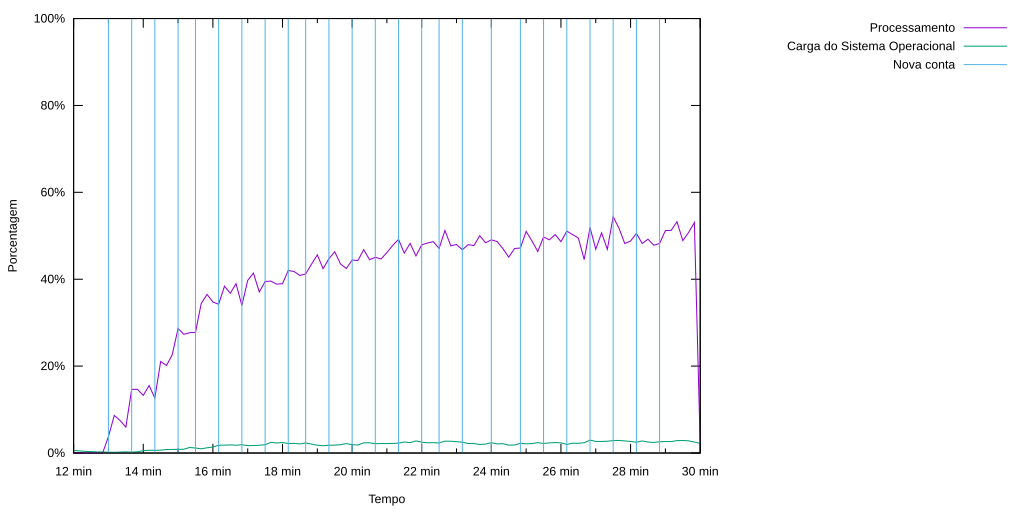
\includegraphics[width=\textwidth]{metricas_rudy_t4/cpu.png}
    \centering
    
    Fonte: O próprio autor
\end{figure}


\section{Consumo de Memória pelo serviço Rudy}

O principal objetivo da coleta de memória da arquitetura Rudy é analisar possiveis vulnerabilidades a qual podem ser sanadas com a escalabilidade do sistema.
%
Em geral, jogos \ac{mmorpg} permitem a divisão de suas regiões em \textit{chunks}, a qual são distribuídos entre os serviços.
%
Esta divisão de carga também é aplicada na arquitetura Rudy.
%
Dessa forma, espera-se que a memória seja impactada pelo número de conexões simultânias em um único pedaço do mundo, consumindo memória para processamento do protocolo \ac{rpc} e armazenamento dos dados do cliente e do mundo, a qual consomem recursos conforme a regra de negócio.

Outro ponto de consumo da memória é referente ao consumo da pilha de execução das chamadas web. Em geral, esta aplicação só consumirá memória especificamente durante a requisição, no qual armazenará o estado no banco de dados, não precisando executar outras operações para manutenção da memória local.
%
Nesse sentido, este teste tende a ter um baixo consumo de memória, visto que as regras de negócio são simples e a memória tende a ser linearmente consumida conforme o número de conexões simultânias.

O teste executado na arquitetura obteve os dados que condizem com a expectativa dos testes, obtendo um baixo consumo de recursos por parte das aplicações da arquitetura Rudy.
%
A Figura~\ref{fig:rudy_t4_memory} compara a memória total com a memória utilizada pela arquitetura.

\begin{figure}[htb!]
    \caption{Registro de memória no servidor utilizando a arquitetura Rudy}
    \label{fig:rudy_t4_memory}
    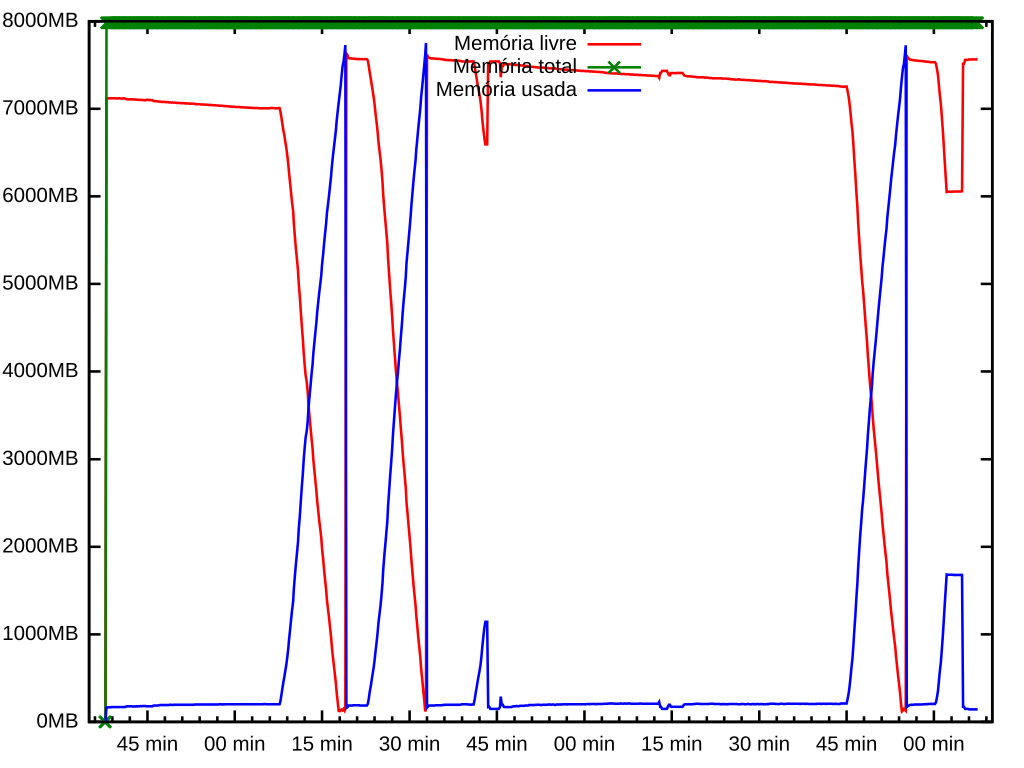
\includegraphics[width=\textwidth]{metricas_rudy_t4/memory.png}
    \centering
    
    Fonte: O próprio autor
\end{figure}

A comparação exibida na Figura~\ref{fig:rudy_t4_memory} mostra somente a escala entre a memória total do serviço com relação a memória consumida.
%
Porém, esta visualização fica comprometida, visto que não fica perceptível a baixa variação da memória consumida com relação ao número de conexões no serviço.
%
A Figura~\ref{fig:rudy_t4_memory_used} trata a escala e aplica somente os dados da memória utilizada pela arquitetura.

\begin{figure}[htb!]
    \caption{Memória consumida no servidor utilizando a arquitetura Rudy}
    \label{fig:rudy_t4_memory_used}
    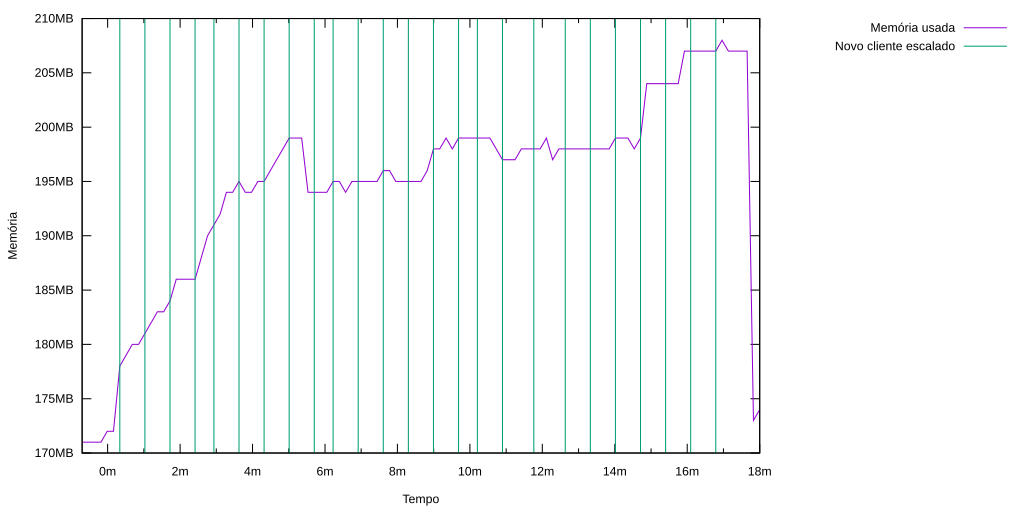
\includegraphics[width=\textwidth]{metricas_rudy_t4/memory_used.png}
    \centering
    
    Fonte: O próprio autor
\end{figure}

Após o tratamento, torna-se notório o crescimento da memória conforme o número de conexões, utilizando uma alícoda de valor pequeno, se comparado ao recurso disponível.
%
Nesse sentido, não foi possível estressar a memória do serviço como um recurso crítico para os testes, porém isto não invalida estes dados para futura comparação com as demais arquiteturas.

\section{Consumo de Banda pelo serviço Rudy}

O principal objetivo do monitoramento do consumo da banda pelo serviço Rudy é verificar se a rede está enfileirando as requisições nos serviços \ac{rpc} na arquitetura.
%
Esta validação é feita caso a rede tenha um limite notório na entrada e saída da rede e o aumento do tempo de requisição, sem comprometer a \ac{cpu} do serviço.

Caso as requisições sejam enfileiradas internamente pelo microsserviço \ac{rpc} (Gerente de Jogo), como o modelo de processamento de requisições da arquitetura Rudy propõe, espera-se que o tempo de resposta que aumente.
%
O aumento do tempo de resposta é um reflexo da concorrência para escrever a requisição \ac{rpc} na fila de processamento do serviço, a qual dependerá do escalonador de threads escolher qual processo escreverá a sua requisição na fila.

Com os dados da banda da arquitetura Rudy obtidos do teste, pode-se observar que o crescimento do consumo da rede não é linear.
%
Os dados podem ser visualizados na Figura~\ref{fig:rudy_t4_io}.

\begin{figure}[htb!]
    \caption{Consumo de Banda no servidor utilizando a arquitetura Rudy}
    \label{fig:rudy_t4_io}
    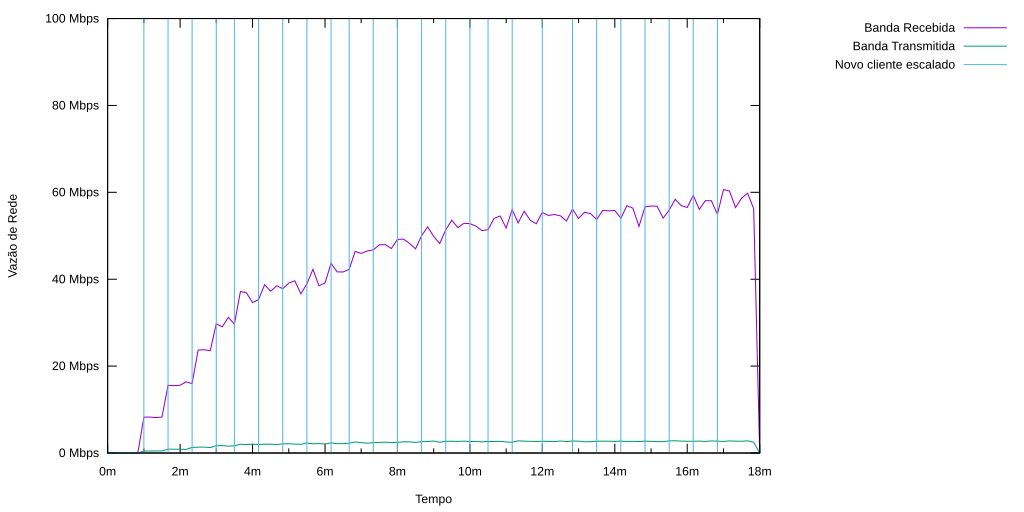
\includegraphics[width=\textwidth]{metricas_rudy_t4/io.png}
    \centering
    
    Fonte: O próprio autor
\end{figure}

Como observado na Figura~\ref{fig:rudy_t4_io}, existe um limite de crescimento da banda.
%
Com as configurações do ambiente, este valor tende a 60Mbps.
%
Vale ressaltar que este gargalo não é proveniente da rede (a qual ficou limitada em 100Mbps), visto que a métrica de latência ficou constante durante os testes.
%
Dessa forma, esta tendência pode ser pela concorrência a fila de processamento, a qual espera-se confirmar com o tempo de resposta do cliente.

\section{Tempo de Resposta pelo cliente Rudy}

Para a arquitetura Rudy, o tempo de resposta do cliente irá confirmar se o enfileiramento das requisições \ac{rpc} ocorreram como previsto.
%
Nesse sentido, espera-se que o tempo de requisição aumente de forma superlinear conforme o número de clientes escalados aumente.


Além disso, será possível visualizar o impácto de operações realizadas no banco com o tempo de resposta do serviço, visto que ao efetuar uma operação no banco a mensagem será transmitida pelos microsserviços web dinâmico e pelo gestor do banco de dados, além do banco de dados por fim.
%
Este impácto chamadas sobre o protocolo \ac{http} com múltiplas camadas deve ser notório conforme a demanda de usuários, atrapalhando o gestor de rede com o consumo de \ac{cpu} e rede para atende-los.

Para comparação entre as requisições \ac{rpc} e web, a Figura~\ref{fig:rudy_t4_reqs} exibe ambas em uma única Figura.
%
Espera-se mostrar o crescimento superlinear das requisições \ac{rpc}, a qual chegam a ultrapassar o tempo de resposta das requisições \ac{http} com múltiplas camadas.

\begin{figure}[htb!]
    \caption{Tempo de Resposta do cliente servidor utilizando a arquitetura Rudy}
    \label{fig:rudy_t4_reqs}
    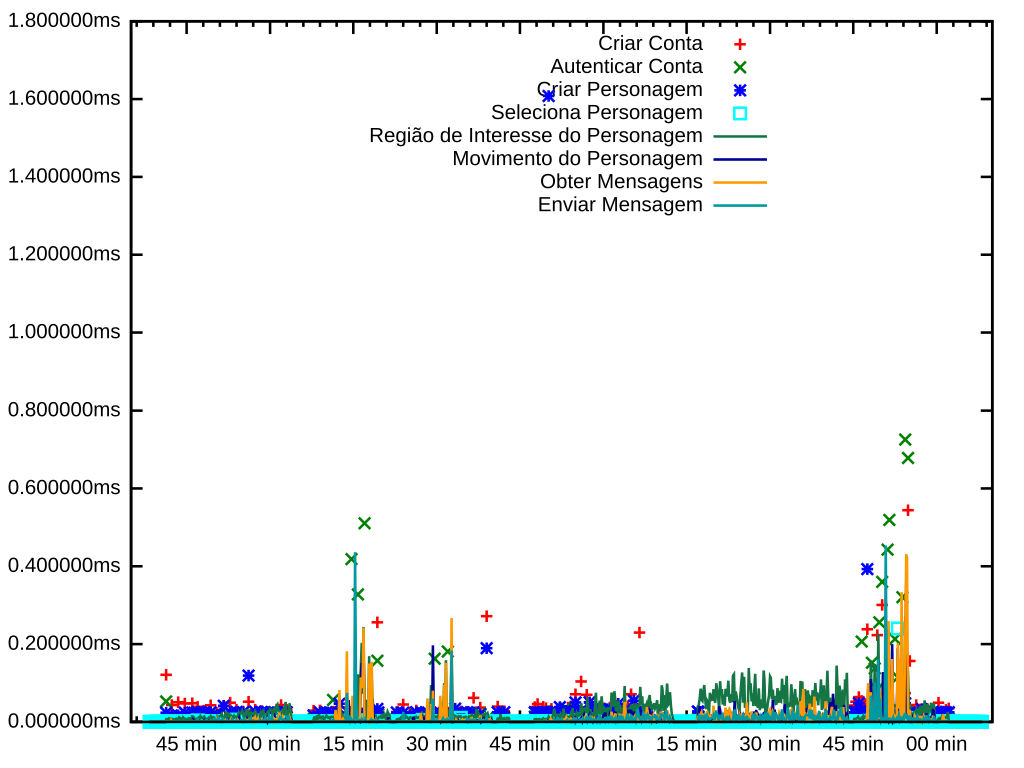
\includegraphics[width=\textwidth]{metricas_rudy_t4/rudyc.png}
    \centering
    
    Fonte: O próprio autor
\end{figure}

A Figura~\ref{fig:rudy_t4_reqs} mostra, dentro de um intervalo de tempo, o tempo de resposta categorizado conforme a ação realizada pelo cliente no serviço.
%
Para facilitar a visualização, este gráfico foi dividido em duas categorias, segregando as requisições sobre \ac{http} e sobre \ac{rpc}.
%
A Figura~\ref{fig:rudy_t4_reqs_https} exibe o tempo de resposta das requisições web em relação ao tempo.
%
Mostra-se na figura a dispersão que ocorre nos tempos de requisições sobre o protocolo \ac{http} conforme o recurso do serviço é consumido por novos clientes.
 

\begin{figure}[htb!]
    \caption{Tempo de Resposta de requisições \textit{Web} do cliente servidor utilizando a arquitetura Rudy}
    \label{fig:rudy_t4_reqs_https}
    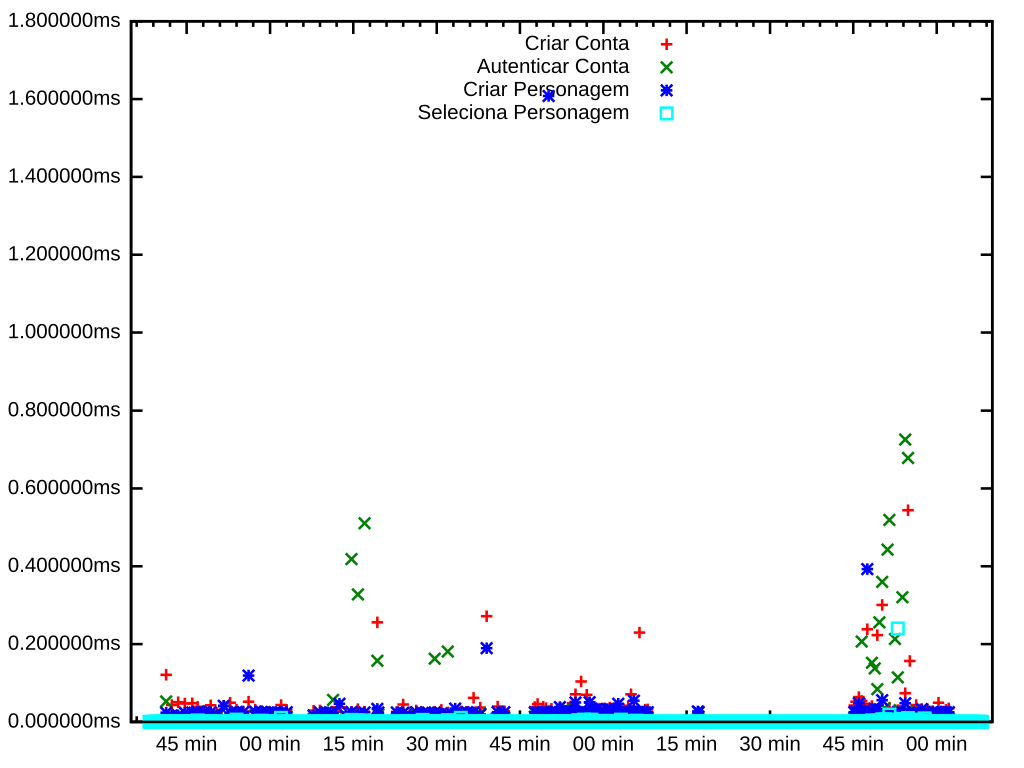
\includegraphics[width=\textwidth]{metricas_rudy_t4/rudyc_http.png}
    \centering
    
    Fonte: O próprio autor
\end{figure}

A Figura~\ref{fig:rudy_t4_reqs_https} exibe uma dispersão conforme o número de conexões do serviço aumenta.
%
Entretanto, espera-se que este tempo de requisição sobre o protocolo \ac{http} aumente somente como um reflexo do consumo de \ac{cpu} e banda pelos clientes.
%
Por este motivo, é notório a necessidade de exibir a parte o tempo de requisição das chamadas \ac{rpc}.
%
Os dados do protocolo \ac{rpc} podem ser visualizados na Figura~\ref{fig:rudy_t4_reqs_rpc}.

\begin{figure}[htb!]
    \caption{Tempo de Resposta de requisições \ac{rpc} do cliente servidor utilizando a arquitetura Rudy}
    \label{fig:rudy_t4_reqs_rpc}
    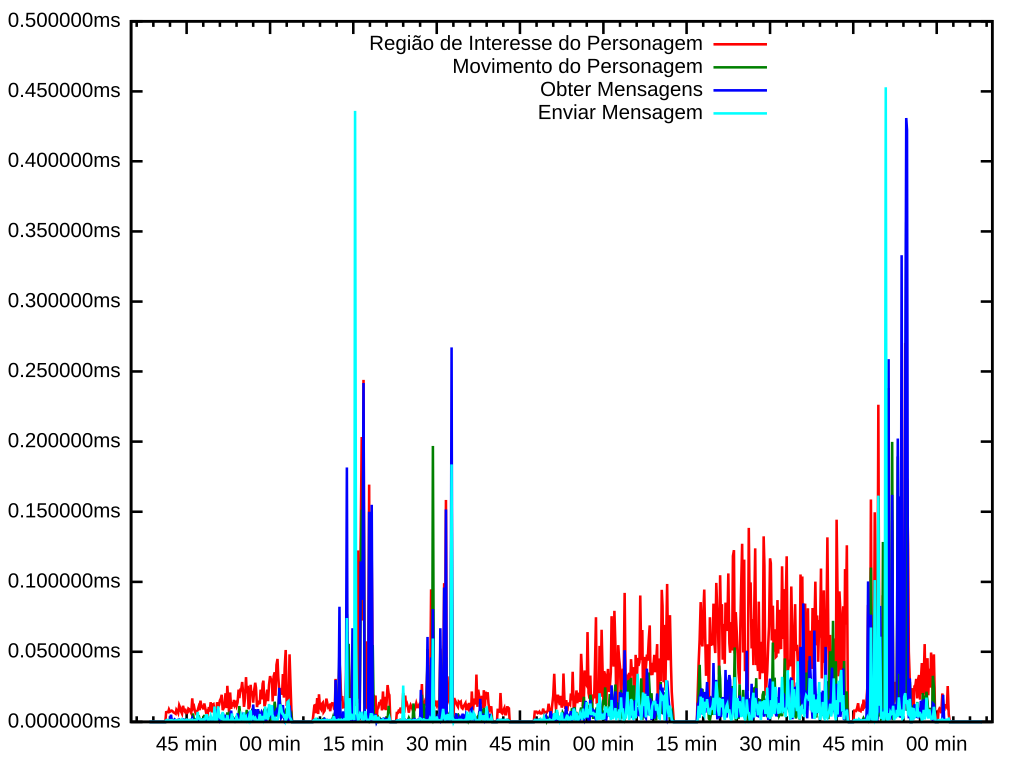
\includegraphics[width=\textwidth]{metricas_rudy_t4/rudyc_rpc.png}
    \centering
    
    Fonte: O próprio autor
\end{figure}

A Figura~\ref{fig:rudy_t4_reqs_rpc} exibe o desparelhamento provocado pelo sistema de filas implementado nesta arquitetura nos serviços \ac{rpc}.
%
Percebe-se também que esta disparidade aumenta diretamente com as requisições \ac{http} ao escalar um novo cliente.
%
Estas informações indicam que de fato ocorre o enfileiramento das requisições, além disso a carga das requisições \ac{http} agravam o enfileiramento, aumentando significantemente o tempo de resposta durante os próximos segundos após a chamada \ac{http}.